\subsection{Задание 1. Простые и сложные сигналы и их свойства}
В этом задании рассматриваются особенности простых и сложных
сигналов, которые проявляются в поведении спектров сигналов. Следует
проследить за тем, какие существуют закономерности при изменении спектров
в зависимости от изменения временных параметров простых и сложных
сигналов.
Для каждого рассмотренного сигнала $m(t)$ строятся графики реализации
сигнала, амплитудного и фазового спектров, а так же функция корреляции и
спектральная плотность энергии.

\textbf{На что ответить в отчете:}
\begin{enumerate}
    \item Получить оценку энергии импульса разными способами по
    экспериментальным данным. Сравнить результаты с
    теоретическими.
    \item \textbf{Done, надо пояснения} Для всех четырех видов сигнала оценить базу,
    используя формулу
    $B=T \cdot \Delta f$, где T - эффективная длительность, $\Delta f$ - эффективная
    ширина полосы спектра сигнала. За оценку ширины следует
    принять половину расстояния между первыми нулями (ширины
    главного лепестка).
    \item Пояснить, как изменяется фазовый спектр сигнала, в том диапазоне
    частот, где лежит основная энергия сигнала. Показать с помощью
    рисунка, как происходит сложение гармонических составляющих
    сигнала. Выделить на графиках амплитудного и энергетического
    спектров диапазон частот, в котором лежит основная энергия
    сигнала. Как изменяется фазовый спектр сигнала в этом диапазоне
    частот? Почему физический амплитудный спектр имеет смысл
    рассматривать только внутри этой полосы?
    \item \textbf{Done, надо пояснения} Для ЛЧМ сигнала сравнить протяженность корреляционной
    функции с длительностью сигнала. Во сколько раз она меньше
    длительности сигнала?
    \item \textbf{Done, надо пояснения} Для ЛЧМ сигнала оценить диапазон изменения фазовых сдвигов у
    гармоник сигнала в пределах полосы амплитудного спектра.
    Нарисовать амплитудный спектр в приближенном виде
    (аппроксимируя прямоугольником) и посмотреть, какой в этих
    пределах фазовый спектр.
    \item Во всех примерах рассматривались изменения спектральных
    характеристик при изменении временных зависимостей сигналов.
    Учитывая, что для функций, сопряженных по Фурье, справедливы
    следующие соотношения (см. Приложение)...(см методичку)
    \item Чем определяется максимальное значение функции корреляции?
    Рассмотреть корреляционную функцию как сигнал и найти его базу.
    \item Сравнить изменения спектрально-корреляционных характеристик
    при изменении длительности различных сигналов.
\end{enumerate}


\subsubsection{Прямоугольный видеоимпульс}
Для прямоугольного видеоимпульса
\begin{itemize}
    \item Получить аналитическое выражение для амплитудного, фазового и
    энергетического спектра, построить теоретический график.
    \item Изучить амплитудный, фазовый и энергетический спектры. Для этого
    задать длительность импульса 10мс и 20мс, амплитуду равной 1, а затем
    проанализировать зависимости.
\end{itemize}

\begin{figure}[H]
    \centering
    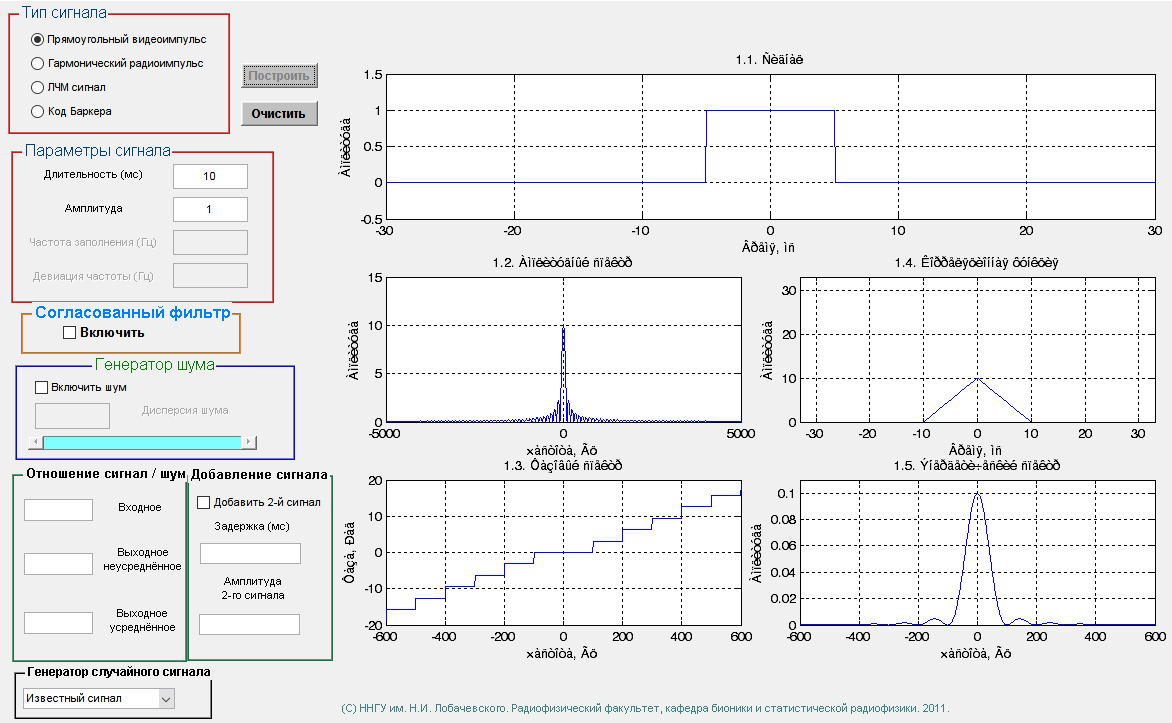
\includegraphics[width=0.9\linewidth]{imgs/t1s1_10.png}
    \caption{10ms}
    \label{fig:task1_10}
\end{figure}
\begin{figure}[H]
    \centering
    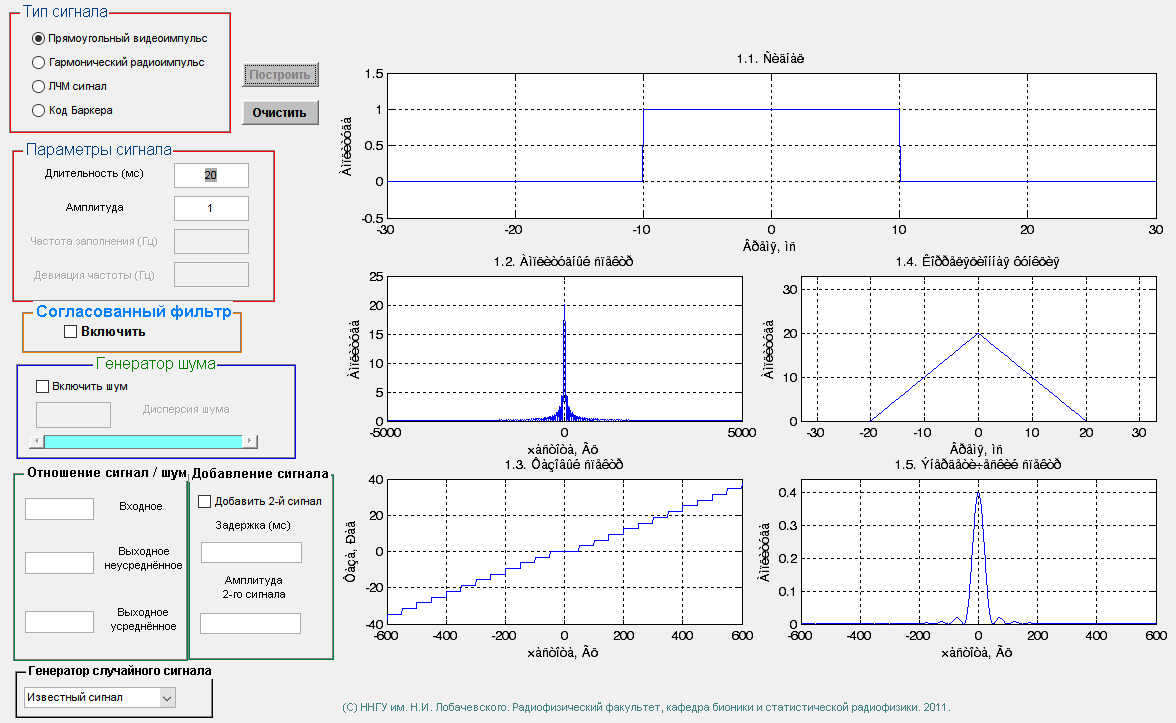
\includegraphics[width=0.9\linewidth]{imgs/t1s1_20.png}
    \caption{20ms}
    \label{fig:task1_20}
\end{figure}

\textit{База}

Найдем базу для прямоугольного импульса по следующей формуле: 
\begin{equation}
    B = T \cdot \Delta f,
    \label{eq:p:1}
\end{equation}
где $T$ - эффективная длительность, $\Delta f$ - эффективная ширина полосы спектра
сигнала(в качестве оценки берется половина ширины главного лепестка амплитудного спектра).
\begin{equation}
    B_{10ms} = 10^{-2} \cdot 100 = 1, \quad B_{20ms} = 20 \cdot 10^{-3} \cdot 50 = 1
    \label{eq:}
\end{equation}
База прямоугольного импульса равна единице, что означает что это простой сигнал. Таким образом
справедливо соотношение $\Delta f = \frac{1}{T}$. Действительно, в соответствии с этой зависимостью,
наблюдается сужение амплитудного спектра при увеличении длительности сигнала.

\textit{Спектры}

Фазовый спектр ??, энергетический спектр так же сузился.

\textit{Энергия}

Получим оценку энергии импульса. Для этого необходимо взять частотный диапазон, в котором фаза $\phi$ спектральных компонент
равна нулю(откуда это и почему ??). В случае прямоугольного импульса (см. рис. \ref{fig:task1_10}), $\phi=0, f \in [-100,
100]$ Гц. 
Полная энергия сигнала равна $2 \pi T$ (см. формулу 49 методички $\int \epsilon(\omega) d\omega$). Найдем значение
энергии в диапазоне $f \in [-100, 100]$ Гц (с помощью численного вычисления интеграла, (см. формулу 49 методички)).
Получим, что $90.2 \%$ энергии находится в указанном диапазоне.
% e_full = 2 pi T = 0.0628
% e=0.0567
% otno = 90.2%


\subsubsection{Прямоугольный видеоимпульс с гармоническим заполнением}
Изучить амплитудный, фазовый и энергетический спектры. Задать
длительность импульса 10мс и 20мс, амплитуду равной 1 и частоту
заполнения 400Гц, а затем проанализировать зависимости.

\begin{figure}[H]
    \centering
    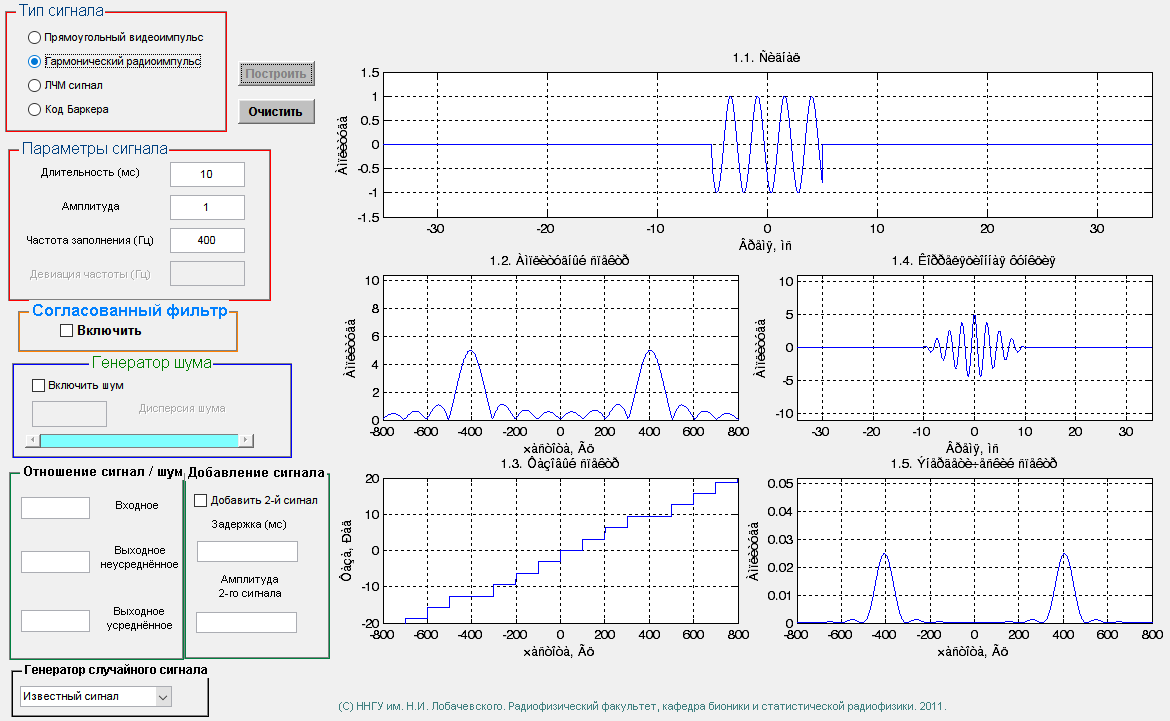
\includegraphics[width=0.9\linewidth]{imgs/t1s2_10.png}
    \caption{10ms}
    \label{fig:task2_10}
\end{figure}
\begin{figure}[H]
    \centering
    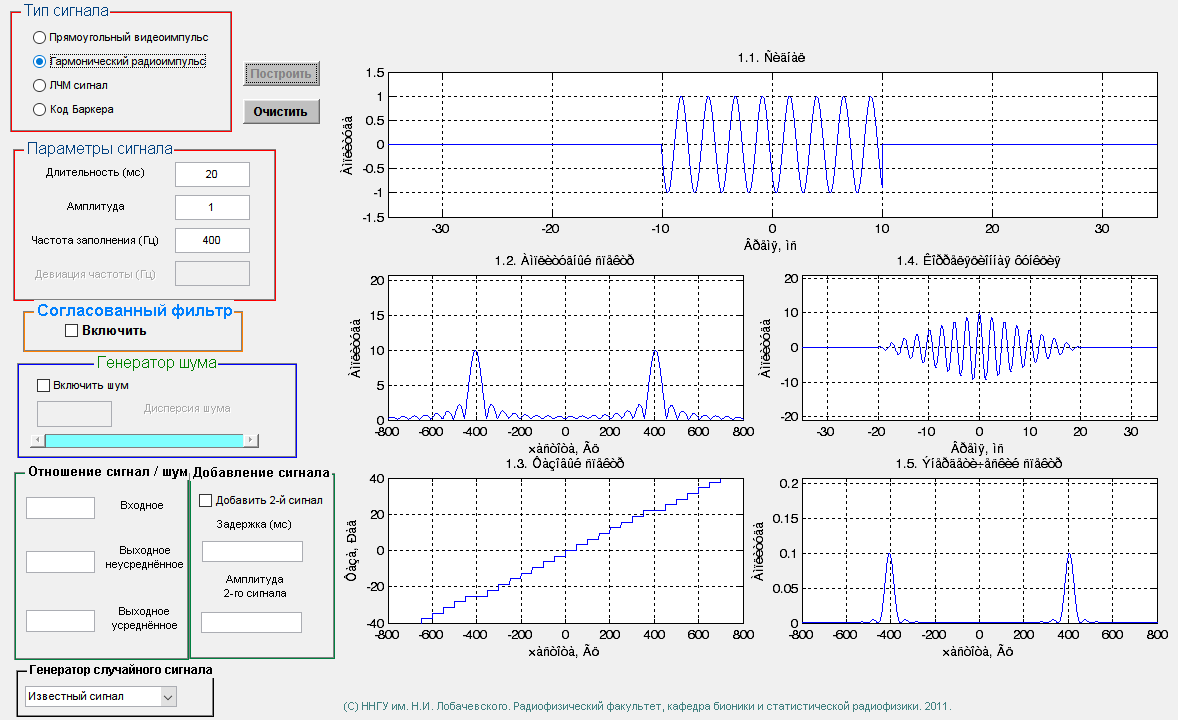
\includegraphics[width=0.9\linewidth]{imgs/t1s2_20.png}
    \caption{20ms}
    \label{fig:task2_20}
\end{figure}
При увеличении длительности сигнала амплитудный спектр ??, фазовый спектр ??, энергетический спектр ??.
\begin{equation}
    B_{10ms} = 10^{-2} \cdot 100 = 1, \quad B_{20ms} = 20 \cdot 10^{-3} \cdot 50 = 1
    \label{eq:}
\end{equation}
Значение базы - единица, означает что радиоимпульс это простой сигнал.

\subsubsection{Линейно-частотный модулированный импульс}
Получить временные реализации ЛЧМ сигнала с параметрами:
\begin{itemize}
    \item длительность 100мс, средняя частота заполнения 1000Гц,
    девиация 500Гц;
    \item длительность 100мс, средняя частота заполнения 1000Гц,
    девиация 1000Гц
    \item амплитуда 1.
\end{itemize}
\begin{figure}[H]
    \centering
    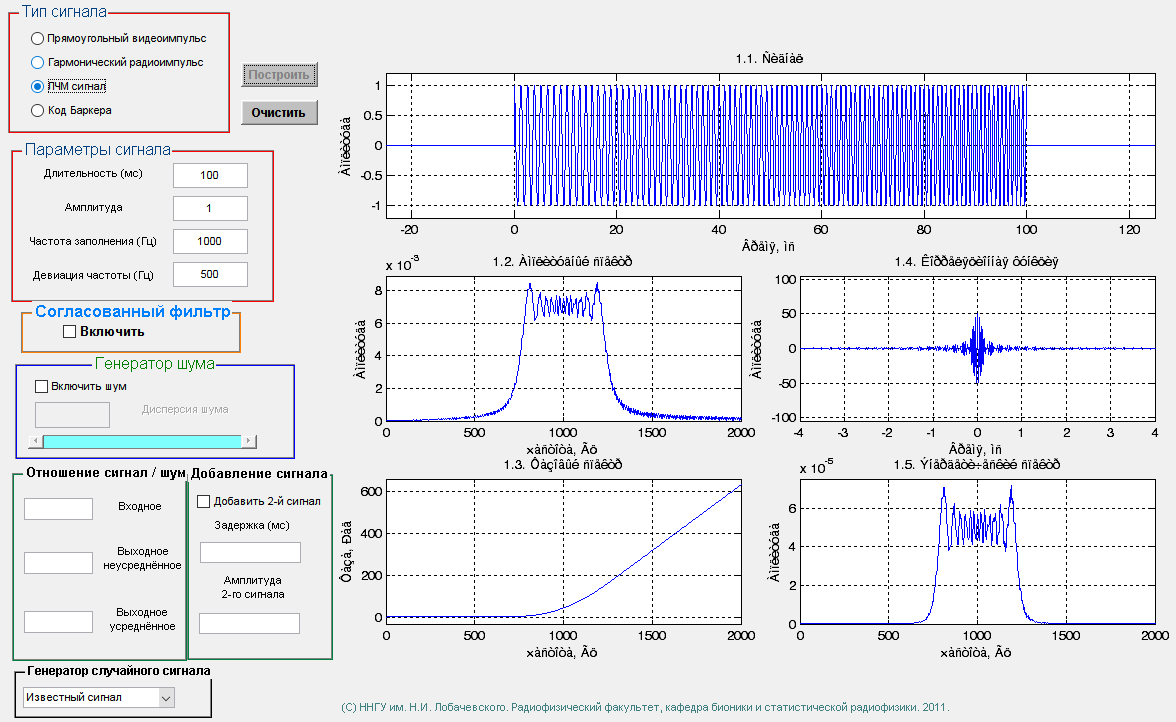
\includegraphics[width=0.9\linewidth]{imgs/t1s3_500.png}
    \caption{500 Гц}
    \label{fig:task3_500}
\end{figure}
\begin{figure}[H]
    \centering
    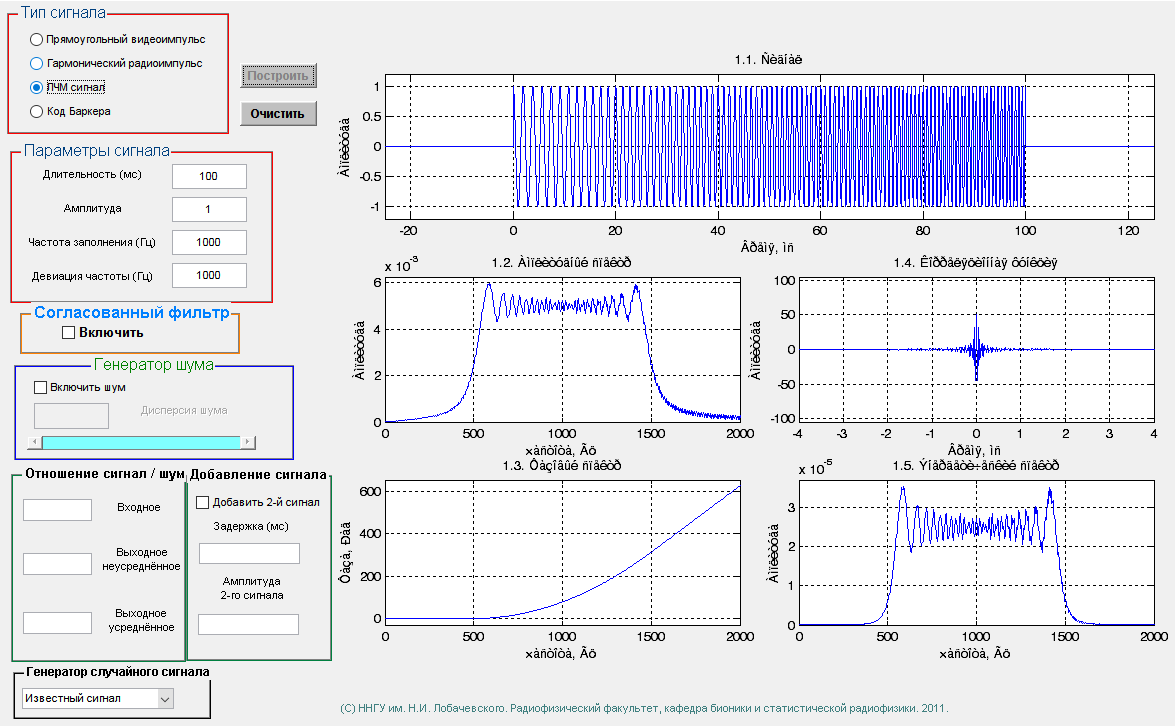
\includegraphics[width=0.9\linewidth]{imgs/t1s3_1000.png}
    \caption{1000 Гц}
    \label{fig:task3_1000}
\end{figure}

\begin{equation}
    B_{500Hz} = 100 \cdot 10^{-3} \cdot (1260-760) = 50, \quad B_{1000Hz} = 100 \cdot 10^{-3} \cdot (1500-500) = 100
    \label{eq:}
\end{equation}

\textbf{Для ЛЧМ сигнала сравнить протяженность корреляционной
функции с длительностью сигнала. Во сколько раз она меньше
длительности сигнала?}

При длительности ЛЧМ сигнала 100 мс, протяженность функции корреляции составила всего 0.4 мс, что в 250 раз меньше.

\textbf{Для ЛЧМ сигнала оценить диапазон изменения фазовых сдвигов у
гармоник сигнала в пределах полосы амплитудного спектра.
Нарисовать амплитудный спектр в приближенном виде
(аппроксимируя прямоугольником) и посмотреть, какой в этих
пределах фазовый спектр.}

Диапазон изменения фазовых сдвигов в случае девиации 500 Гц составил $\phi \in [0 - 160]$ радиан (см. рис.
\ref{fig:task3_500_phase}), в случае девиации 1000 Гц составил $\phi \in [0 - 260]$ радиан (см. рис.
\ref{fig:task3_1000_phase}).
\begin{figure}[H]
    \centering
    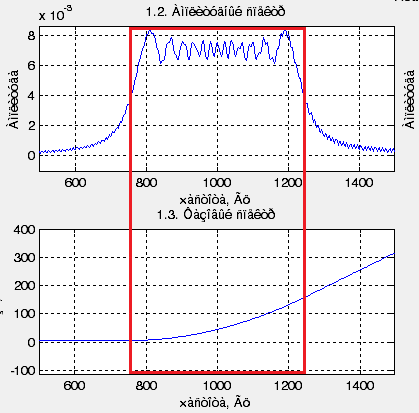
\includegraphics[width=0.5\linewidth]{imgs/t1s3_500_extra.png}
    \caption{Диапазон изменения фазовых сдвигов у гармоник сигнала, девиация 500 Гц}
    \label{fig:task3_500_phase}
\end{figure}

\begin{figure}[H]
    \centering
    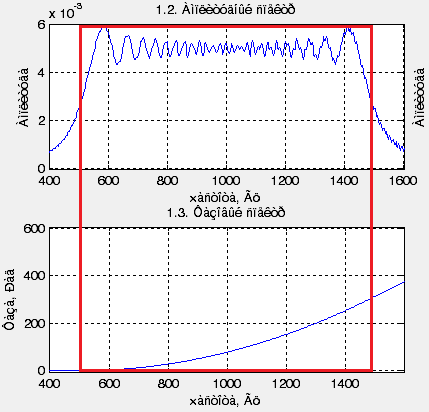
\includegraphics[width=0.5\linewidth]{imgs/t1s3_1000_extra.png}
    \caption{Диапазон изменения фазовых сдвигов у гармоник сигнала, девиация 1000 Гц}
    \label{fig:task3_1000_phase}
\end{figure}

\subsubsection{Код Баркера}
Получить реализации для кода Баркера (N=13) при длительности 13мс и
26мс
\begin{figure}[H]
    \centering
    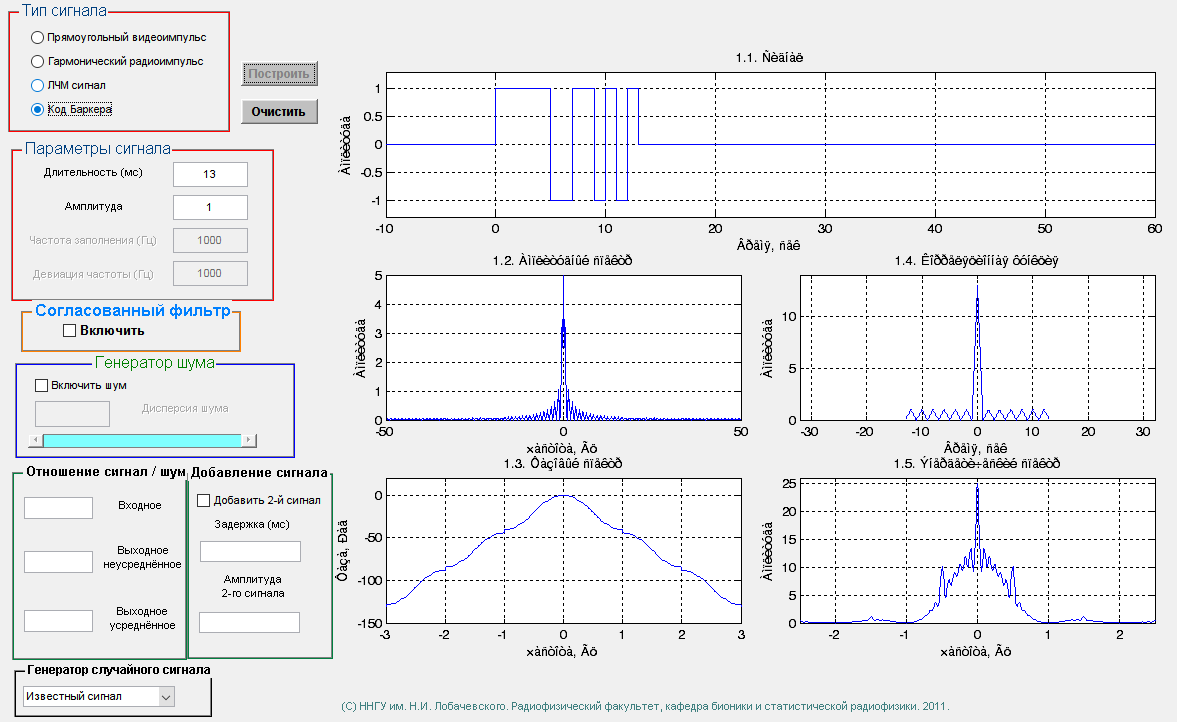
\includegraphics[width=0.9\linewidth]{imgs/t1s4_13.png}
    \caption{13 мс}
    \label{fig:task4_13}
\end{figure}
\begin{figure}[H]
    \centering
    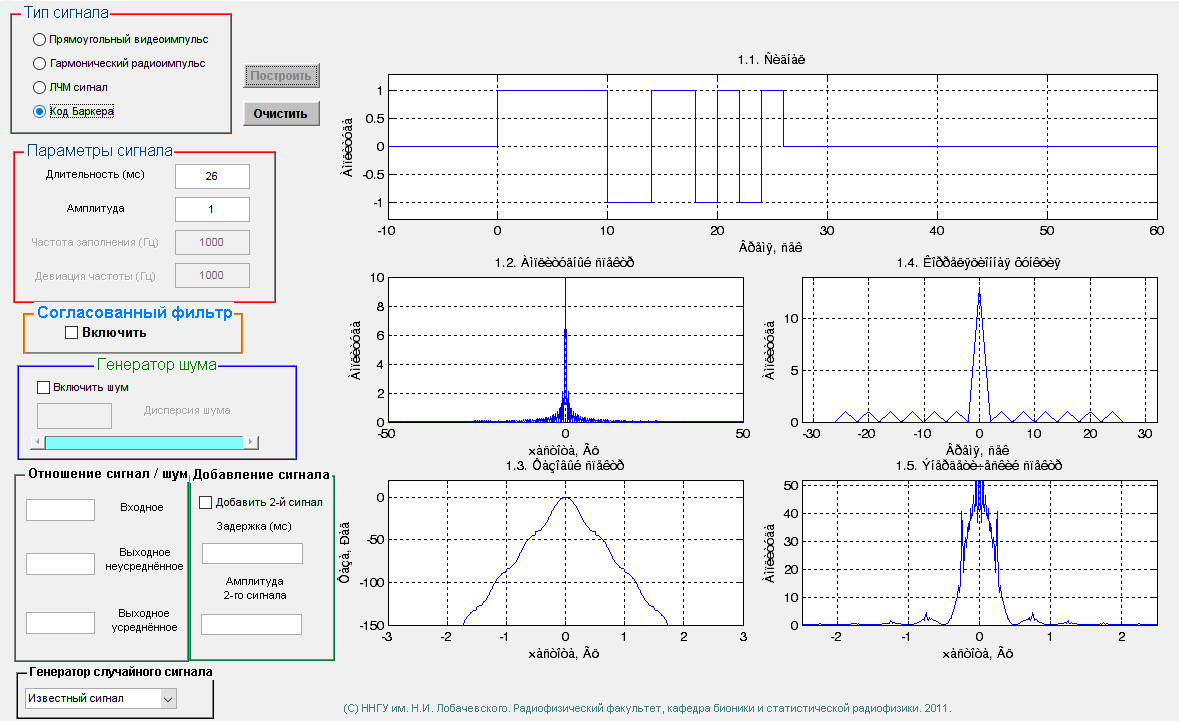
\includegraphics[width=0.9\linewidth]{imgs/t1s4_26.png}
    \caption{26 мс}
    \label{fig:task4_26}
\end{figure}

\begin{equation}
    B_{13ms} = 13 \cdot 10^{-3} \cdot 1 = 13 \cdot 10^{-3}, \quad B_{26ms} = 26 \cdot 10^{-3} \cdot 0.5 = 13 \cdot 10^{-3}
    \label{eq:}
\end{equation}
